\chapter{Estado de la cuestión}

Esta sección tiene como objetivo analizar los algoritmos de timetabling existentes y sus aplicaciones en el ámbito universitario. Se discutirán las ventajas y limitaciones de las soluciones actuales y otros trabajos relacionados.\newpage

\section{Algoritmos de timetabling}

El \textbf{timetabling} puede definirse generalmente como la actividad de asignar, con sujeción a restricciones, una serie de eventos a un número limitado de periodos de tiempo y lugares, de forma que se satisfagan los objetivos deseables en la medida de lo posible. Los casos prácticos en los que se plantea esta actividad son muy variados. En el ámbito educacional, empresarial, deportivo, de comunicación y transporte, entre otros \cite{hybrid-timetabling}.\newline

Generalmente, en las instituciones de enseñanza son dos los problemas de timetabling que surgen: uno para \textbf{exámenes} (Examination Timetabling Problem) y el otro para la \textbf{programación de cursos} (Course Timetabling Problem y Class/Teacher Timetabling Problem o CTTP) \cite{carter}.\newline

\subsection{Examination Timetabling Problem}
El ETP básicamente involucra la asignación de una serie de exámenes a un período de examinación dado. Algunas versiones de este problema requieren que el calendario de la solución use el mínimo número de períodos de tiempo. Cada ETP tiene su propio conjunto de restricciones duras y restricciones blandas \cite{AutomatedTimetabling} \cite{NAJIAZIMI2005705}.\newline

Las restricciones duras deben ser satisfechas por el calendario. Por ejemplo, un estudiante no puede tener dos exámenes al mismo tiempo. Los calendarios que cumplen las restricciones duras se conocen como ``calendarios factibles''.\newline

Los requisitos blandos, por otra parte, son una lista de deseos con propiedades que se querría que los calendarios posean. Por ejemplo, no se acumularán en un mismo día varios exámenes de elevada dificultad y duración.\newline

El enfoque adoptado por los primeros intentos de resolver el ETP generalmente consistía en clasificar los exámenes según la dificultad asociada a la programación de los mismos y ordenando a estos como los primeros para evitar que se produjesen solapamientos. Desde entonces, múltiples avances se han producido en la resolución de este problema, incluyendo la aplicación de heurísticas y metaheurísticas, técnicas de construcción secuencial, algoritmos genéticos, etc.\newpage

A continuación se muestra un ejemplo de un algoritmo genético\footnote{Algoritmo Genético Interactivo (por sus siglas en inglés, Interactive Genetic Algorithm). Los IGAs son una variación de los algoritmos genéticos tradicionales que involucran la interacción humana en el proceso de optimización.} para resolver el ETP \cite{PILLAY2010457}:

\begin{figure}[H]
    \centering
    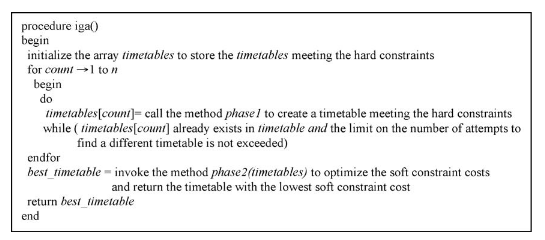
\includegraphics[width=1\textwidth]{./imagenes/IGA_ETP.png}
    \caption{Ejemplo de IGA para evolucionar calendarios ``factibles'' \cite{PILLAY2010457}.}
\end{figure}

\newpage

% \newpage

% \begin{figure}
%     \begin{figure}[H]
%         \centering
%         \rotatebox{90}{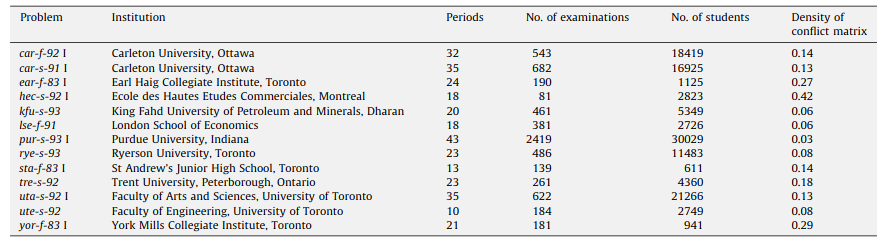
\includegraphics[width=1.5\textwidth]{./imagenes/IGA_Carter_Benchmarks.png}}
%         \caption{Benchmarks en los que fue probado el algoritmo de la figura anterior\cite{PILLAY2010457}.}
%     \end{figure}
% \end{figure}

\subsection{University Course TimeTabling Problem}

El UCTTP, es un problema de optimización\footnote{Es un problema que trata de calcular el valor máximo o mínimo de una función, en nuestro caso, de una variable. Por ejemplo: minimizar el error en una medición, minimizar la cantidad de material para construir un contenedor, maximizar el volumen de un contenedor, minimizar el tiempo de espera o de recorrido, etc.} híbrido que se presenta al comienzo de cada semestre de las universidades e incluye la asignación de eventos(\textbf{cursos}, profesores y estudiantes) a una serie de \textbf{franjas horarias} y salas fijas. Este problema debe satisfacer tanto las restricciones duras como las blandas durante la asignación de eventos a los recursos\footnote{Son usados por los eventos, tales como: salas, franjas de tiempo, etc.}, de modo que los posibles horarios se obtienen después de la plena satisfacción de todas las restricciones duras y también de las restricciones blandas para aumentar y promover la calidad de los posibles horarios generados según sea necesario \cite{UCTTP_ThreePhaseApproach}.\newline

El número de restricciones (duras y blandas) en este problema difiere de una institución a otra. Por lo tanto, el objetivo principal de todos los algoritmos mencionados es maximizar el número de restricciones blandas satisfechas en los horarios finales \cite{article_1445178}.\newline

Las restricciones del problema se clasifican en dos clases: duras y blandas. Las duras deben satisfacerse por completo en el problema para que la solución generada sea posible y sin conflictos; no se permite ninguna violación de estas restricciones. Las restricciones blandas están relacionadas con la función objetivo; la cual consiste en maximizar el número de restricciones blandas satisfechas. A diferencia de las restricciones duras, las blandas no tienen que satisfacerse necesariamente; pero a medida que aumenta el número de estas restricciones satisfechas, aumenta la calidad de las soluciones de dicha función. A continuación se presenta una lista de ejemplos de restricciones duras y blandas \cite{BABAEI201543}:

\begin{itemize}
    \item Un profesor no puede estar en dos lugares al mismo tiempo.
    \item Una clase no puede impartirse en dos salas al mismo tiempo.
    \item Un profesor imparte solo una clase a la vez.
    \item Un profesor puede solicitar un aula específica para una clase.
    \item El número máximo de horas que un profesor puede impartir en una clase son 4 horas.
    \item El máximo de horas que un alumno puede tener en un día son 4 horas.
    \item La hora de inicio de las clases puede ser las 8:00 a.m y la de finalización las 20:30 p.m. generalmente.
\end{itemize}
A continuación se muestra un ejemplo de un algoritmo para resolver el UCTTP mediante búsqueda iterativa en profundidad:

\begin{figure}[H]
    \centering
    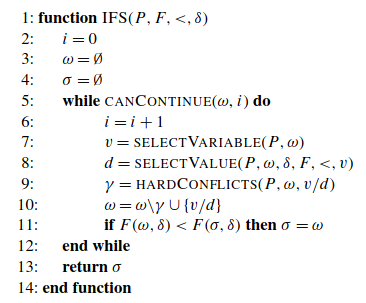
\includegraphics[width=0.7\textwidth]{./imagenes/UCTTP_Algoritmo.png}
    \caption{Pseudocódigo para algoritmo de UCTTP \cite{Rudova2011}.}
\end{figure}

\newpage

\subsection{Class/Teacher Timetabling Problem}

El CTTP, suele encontrarse en escuelas con planes de estudios menos modulares. Tal es el caso de la mayoría de los institutos y algunas universidades, donde la mayoría de las lecciones predefinidas adscritas a cada curso son obligatorias para las respectivas clases. A diferencia del problema de programación de cursos, en el caso del CTTP \textbf{no se permite el solapamiento de lecciones}. En este caso, el objetivo consiste en programar el conjunto de lecciones satisfaciendo una serie de restricciones específicas de la institución \cite{doi:10.1504/IJOR.2024.139234}.\newline

Se han aplicado varias técnicas de resolución, desde
algoritmos basados en la teoría de grafos (de Werra 1996), a la programación binaria (Tri-pathy 1984; Birbas et al. 1997) y enfoques basados en restricciones (Yoshikawa et al. 1994). Además, las metaheurísticas basadas en el recocido simulado (Abramson 1982), las redes neuronales (Gislen et al. 1992), los algoritmos genéticos (Colorni et al. 1991) y la búsqueda tabú (Costa 1994) se han aplicado con éxito a casos concretos, objeto de estudio de los respectivos autores.\newline

En términos generales, el CTTP puede definirse como el problema de programar un conjunto de lecciones (una lección es una asignación previa de una o más clases rígidas de alumnos a un profesor y una asignatura) en un conjunto de periodos de tiempo y aulas adecuadas, satisfaciendo al mismo tiempo una amplia gama de restricciones. Estas pueden dividirse en dos niveles de importancia, como en los problemas de timetabling anteriores: restricciones duras y blandas \cite{carter}.\newpage

\begin{figure}[H]
    \centering
    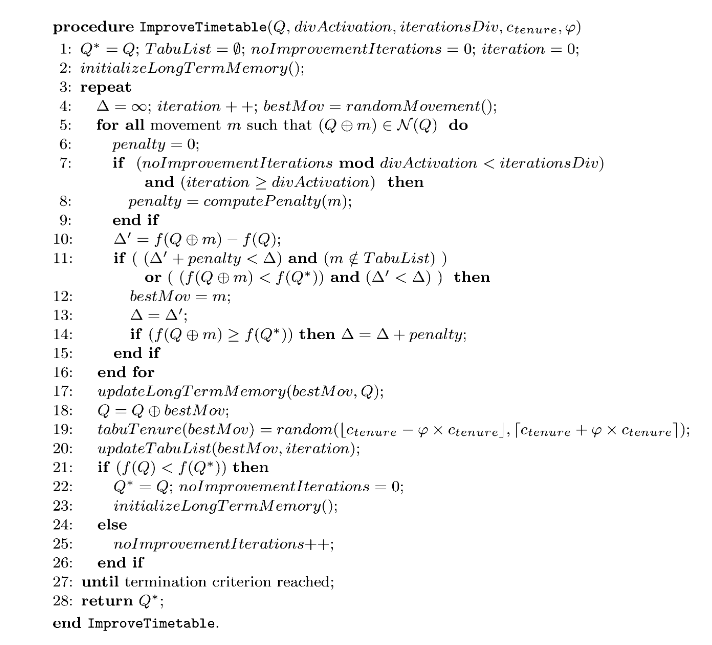
\includegraphics[width=1\textwidth]{./imagenes/CTTP.png}
    \caption{Pseudocódigo del algoritmo de búsqueda tabú para el CTTP \cite{tabuSearch}.}
\end{figure}

\newpage

\begin{landscape}
    

\begin{table}[h!]
    \centering
    \renewcommand{\arraystretch}{1.2}
    \begin{tabular}{|p{4cm}|p{4cm}|p{4cm}|p{4cm}|}
    \hline
    \textbf{Aspecto} & \textbf{Course Timetabling} & \textbf{Class/Teacher Timetabling} & \textbf{Examination Timetabling} \\ \hline
    
    \textbf{Objetivo Principal} & 
    Asignar horarios para cursos sin conflictos y equilibrar la carga semanal. & 
    Asignar horarios específicos a clases individuales y distribuir a los profesores eficientemente. & 
    Programar exámenes evitando conflictos y distribuyendo la carga de estudio. \\ \hline
    
    \textbf{Horizonte Temporal} & 
    Todo el semestre o año académico. & 
    Semanal durante el semestre o año académico. & 
    Periodo de exámenes, típicamente al final de un semestre. \\ \hline
    
    \textbf{Restricciones Clave} & 
    Disponibilidad de aulas, no superposición de cursos, balancear carga semanal de cursos. & 
    Disponibilidad de profesores y aulas, tamaño de clases, continuidad lógica de las clases. & 
    Evitar conflictos de horarios para estudiantes, minimizar exámenes consecutivos, disponibilidad de salas de examen. \\ \hline
    
    \textbf{Nivel de Abstracción} & 
    Macro: planificación de horarios generales para cursos completos. & 
    Micro: planificación de horarios detallados para clases y profesores. & 
    Específico: planificación de horarios de exámenes en un corto período. \\ \hline
    
    \textbf{Recursos Considerados} & 
    Aulas, disponibilidad de cursos. & 
    Aulas, disponibilidad de profesores, tamaño de clases. & 
    Salas de examen, supervisores, recursos específicos para exámenes. \\ \hline
    
    \textbf{Complejidad} & 
    Alta, pero menos que la programación de exámenes debido a un período más largo para distribuir cursos. & 
    Alta, con mayor detalle en la planificación respecto a profesores y clases. & 
    Muy alta, debido a la concentración de eventos en un corto período y la necesidad de evitar solapamientos. \\ \hline
    
    \end{tabular}
    \caption{Comparación entre Course Timetabling, Class/Teacher Timetabling y Examination Timetabling.}
    \label{tab:comparison}
    \end{table}
\end{landscape}
\newpage
\section{Trabajos relacionados}

Para intentar solucionar el problema propuesto al principio del documento hay pocas alternativas existentes. Existen múltiples agendas y calendarios electrónicos que nos permitirían llevar el seguimiento de nuestro calendario semanal, pero no resuelven el problema (al menos de forma automática) de generar todas las combinaciones posibles para poder escoger la que más se adapte a nuestras necesidades.\newline

Voy a apoyarme en un caso práctico, para poder analizar las soluciones disponibles actualmente y poder evaluar el estado de la cuestión:\newline

Llega fin de curso, ya tenemos escogidas las asignaturas que planeamos cursar el próximo año y hemos recopilado de la información de los grupos y subgrupos de cada una de ellas. Sin embargo, las asignaturas se reparten entre 1º, 2º y 3º. Una de ellas necesitamos cursarla en un grupo concreto para convalidar las prácticas que tenemos aprobadas del curso pasado y a ser posible nos gustaría no pasar muchas horas al día en la facultad.

\subsection{Agendas y calendarios virtuales}
A priori la opción más simple y menos práctica. Organizamos los grupos según nuestras preferencias: rellenamos el calendario con el grupo del profesor que nos gustaría que nos convalidase las prácticas y vamos poco a poco, a base de en ensayo y error, introduciendo el resto de grupos y combinándolos para evitar solapamientos.

\subsection{Google Calendar}
Es un servicio de agenda y calendario en línea ofrecido por Google\footnote{\url{https://calendar.google.com/calendar}}.  Permite a los usuarios crear y editar eventos. Los eventos tienen una fecha y hora de inicio y fin, además de una descripción. Los usuarios pueden invitar a otros usuarios a sus eventos, y los eventos pueden ser públicos o privados. Los usuarios pueden ver sus eventos en una vista diaria, semanal o mensual. También permite a los usuarios generar múltiples calendarios y compartirlos con otros usuarios. Los usuarios pueden ver los calendarios de otras personas y superponerlos en su propio calendario. Google Calendar también se integra con otras aplicaciones de Google, como Gmail y Google Meet. Google Calendar también se integra con otras aplicaciones de calendario, como Microsoft Outlook y Apple Calendar. Está disponible en la web y en aplicaciones móviles para Android e iOS.

\begin{landscape}

\begin{figure}[H]
    \centering
    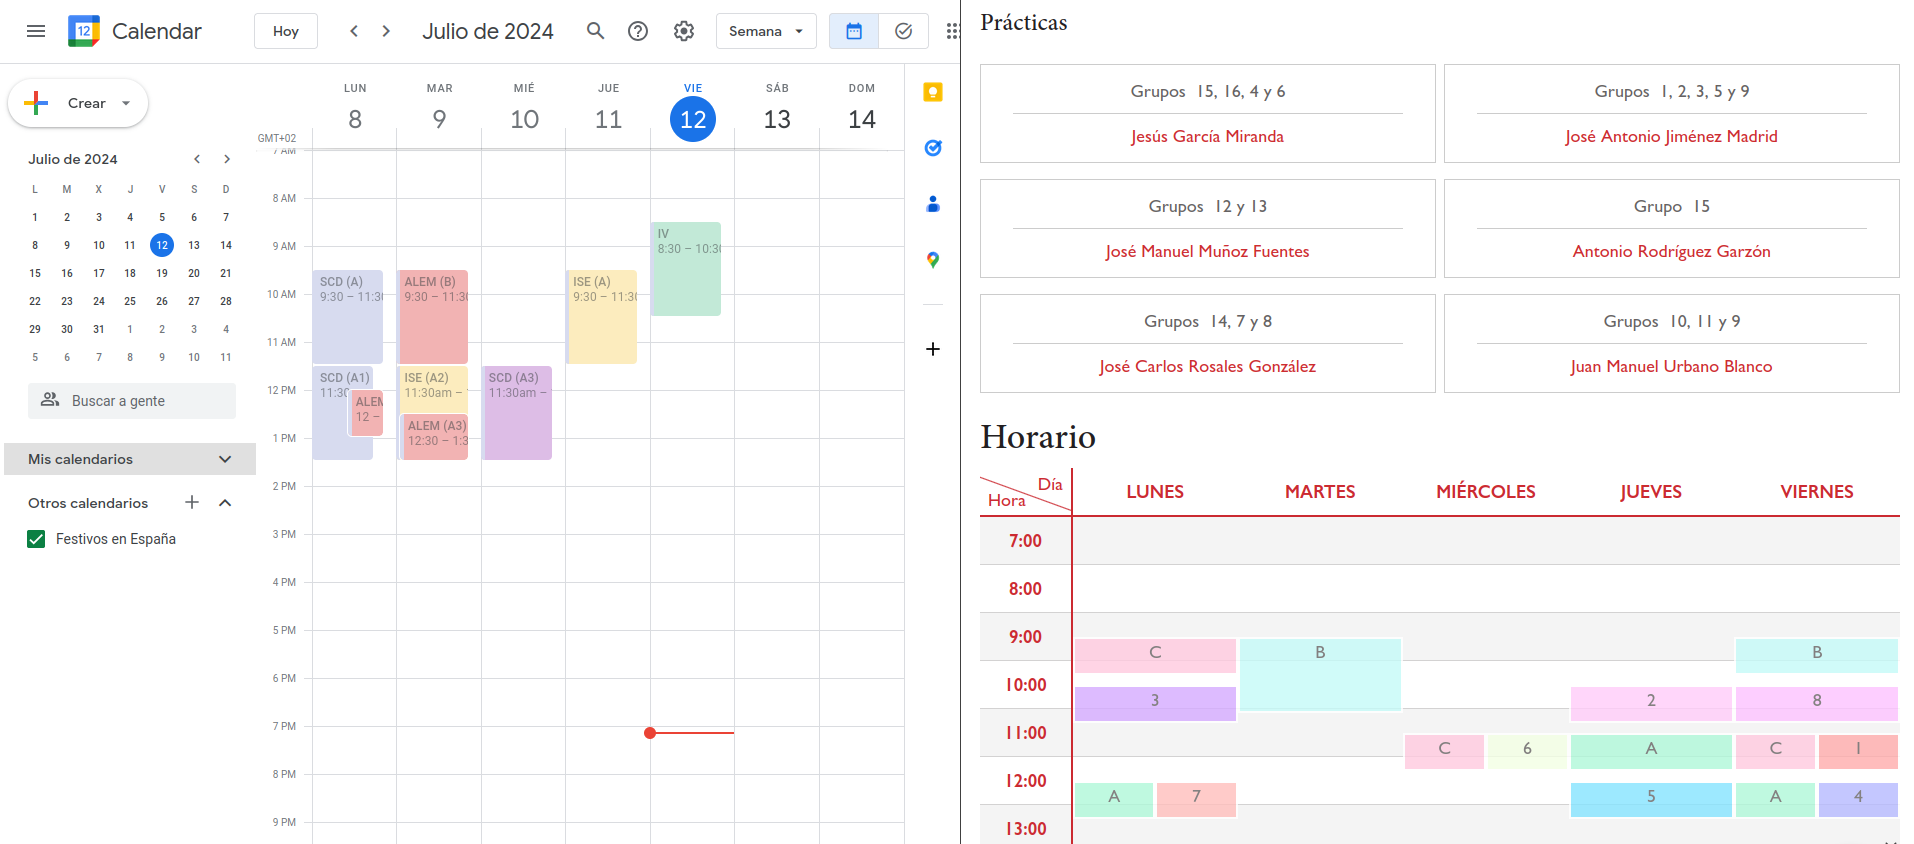
\includegraphics[width=1.5\textwidth, angle=0]{./imagenes/Google_Calendar.png}
    \caption{Ejemplo de uso con Google Calendar.}
\end{figure}

\end{landscape}


\subsection{Microsoft Calendar}
Es una función integrada en aplicaciones como Outlook y Microsoft 365\footnote{\url{https://outlook.live.com/calendar}} que permite a los usuarios gestionar y organizar sus calendarios personales y profesionales. Facilita la creación y edición de citas, reuniones, y eventos, con opciones de recordatorios y notificaciones. Se sincroniza en la nube, ofreciendo acceso desde múltiples dispositivos, y permite compartir calendarios con otros usuarios. Además, se integra con otros servicios de calendario y herramientas de Microsoft, como Teams, facilitando la coordinación en equipos de trabajo y la gestión eficiente del tiempo.

\newpage

\begin{landscape}
\begin{figure}[H]
    \centering
    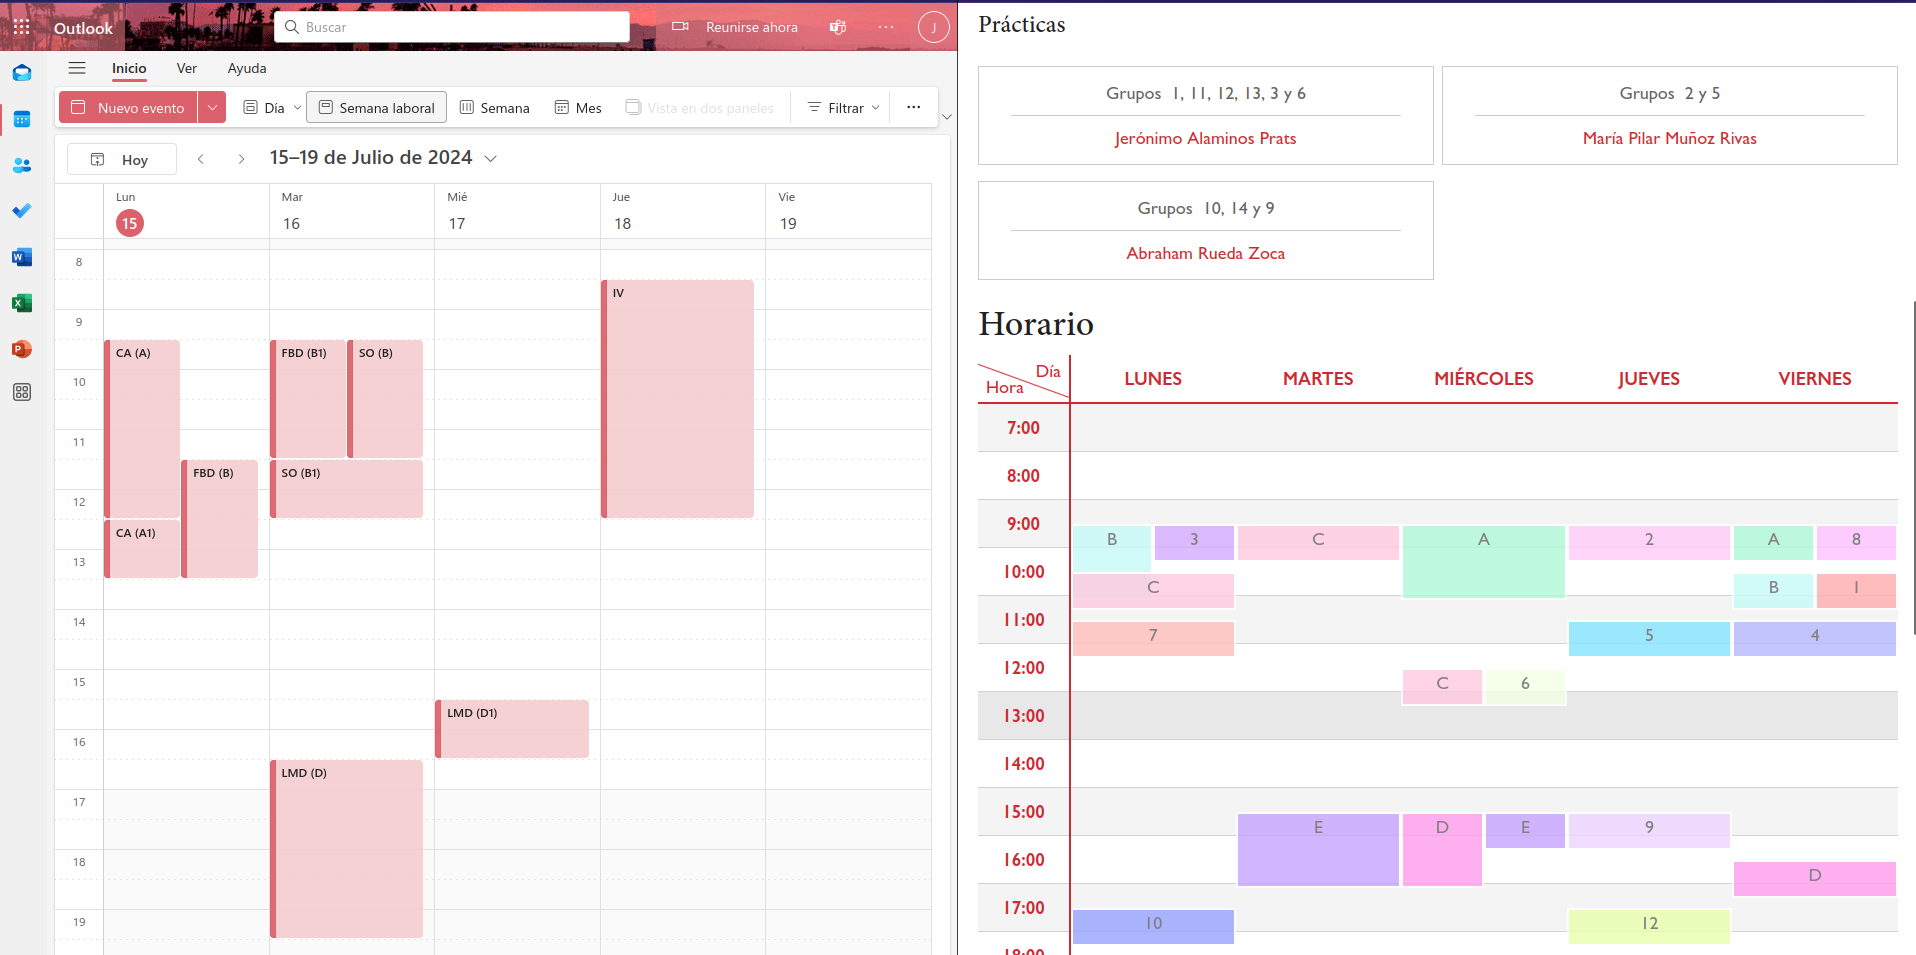
\includegraphics[width=1.5\textwidth, angle=0]{./imagenes/Microsoft_calendar.png}
    \caption{Ejemplo de uso con Microsoft Calendar.}
\end{figure}
\end{landscape}


\subsection{Chatbots}
En un primer momento, era la opción escogida para llevar a cabo este proyecto. Sin embargo, tras varias pruebas con diversos chatbots y modelos como \emph{ChatGPT y Gemini}, se acabó descartando la idea dada la inconsistencia de los asistentes para organizar las clases de forma que no se solaparan y sin alterar los datos de los horarios proporcionados.

\subsubsection*{ChatGPT}
Es un modelo de lenguaje de inteligencia artificial desarrollado por OpenAI\footnote{\url{https://chatgpt.com/}}. Es capaz de mantener conversaciones con los usuarios y responder preguntas en lenguaje natural. ChatGPT se basa en la arquitectura de transformadores y emplea el aprendizaje profundo para generar respuestas coherentes y relevantes. ChatGPT se puede utilizar en una variedad de aplicaciones, como asistentes virtuales, chatbots y sistemas de diálogo. ChatGPT es capaz de responder preguntas sobre una amplia gama de temas y proporcionar información útil a los usuarios. ChatGPT es una herramienta poderosa para la generación de lenguaje natural y la interacción con los usuarios en línea.

\begin{landscape}
    \begin{figure}[H]
        \centering
        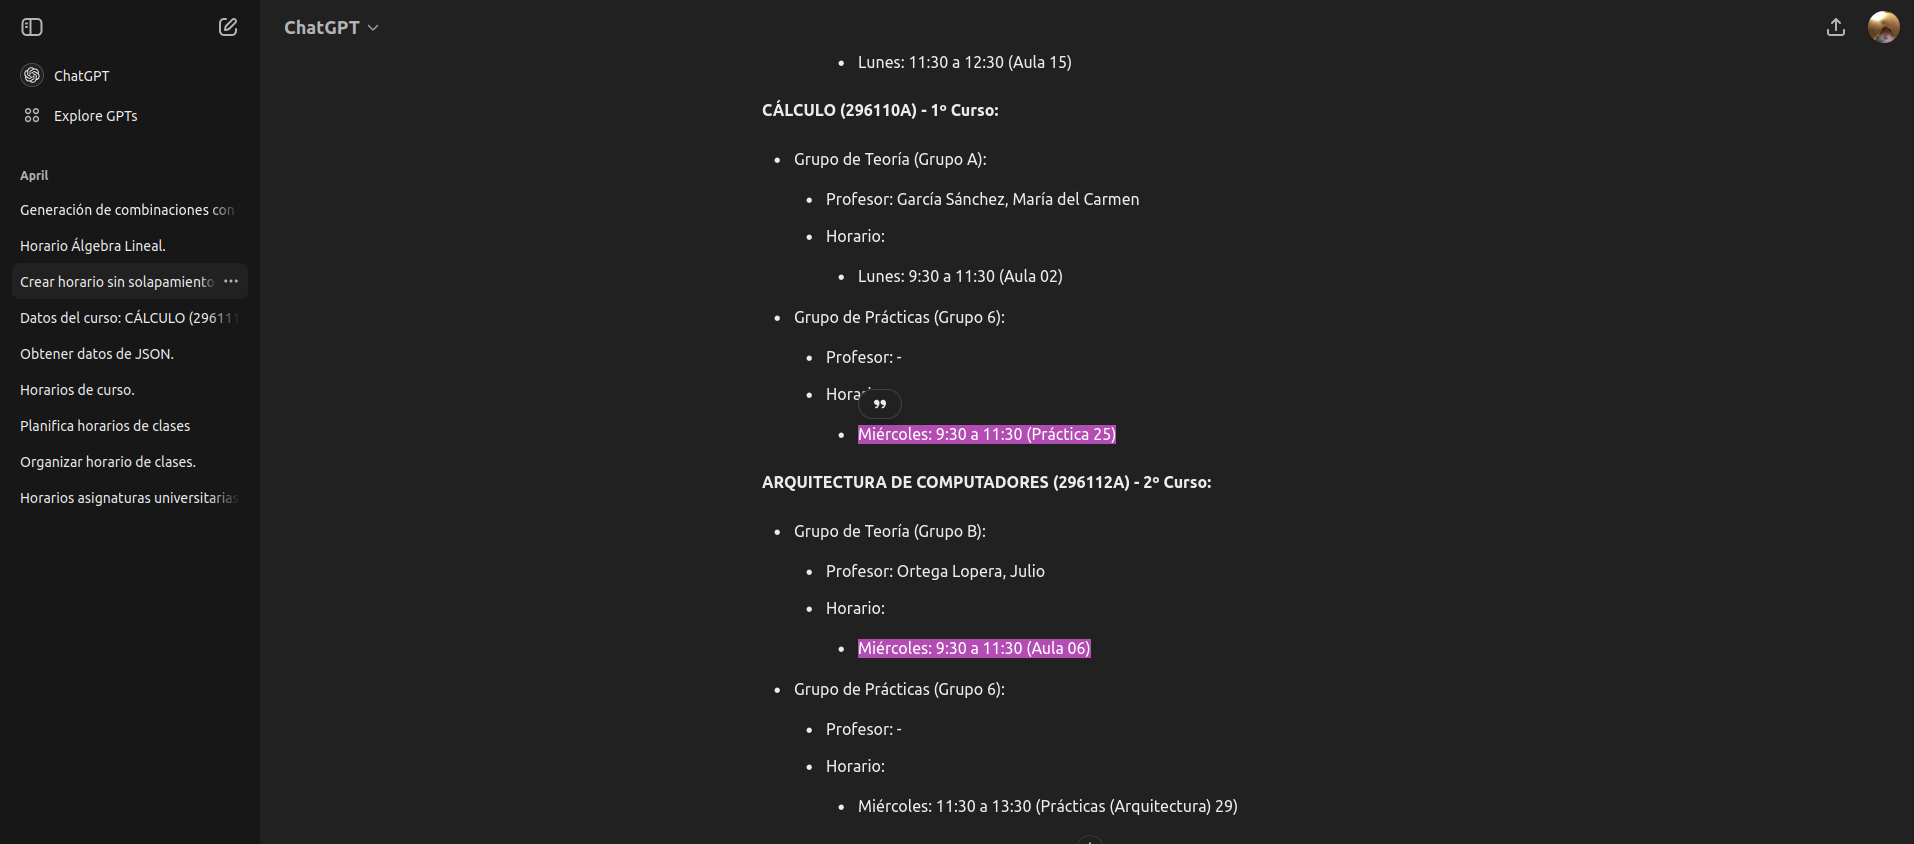
\includegraphics[width=1.5\textwidth, angle=0]{./imagenes/ChatGPT.png}
        \caption{Ejemplo con ChatGPT 3.5: solapa las clases.}
    \end{figure}
\end{landscape}

\subsubsection*{Gemini}
Es una familia de modelos de inteligencia artificial desarrollada por Google DeepMind\footnote{\url{https://gemini.google.com/app}}. Es la evolución de la tecnología detrás de Bard, integrando capacidades avanzadas de procesamiento de lenguaje natural con otros aspectos de la inteligencia artificial, como el razonamiento y la memoria. Gemini está diseñado para realizar tareas complejas que van más allá de la generación de texto, buscando mejorar la comprensión contextual, la generación de respuestas más precisas y la interacción más fluida con los usuarios. Es parte del esfuerzo de Google por mantenerse a la vanguardia en el desarrollo de IA generativa y cognitiva.

\begin{landscape}
    \begin{figure}[H]
        \centering
        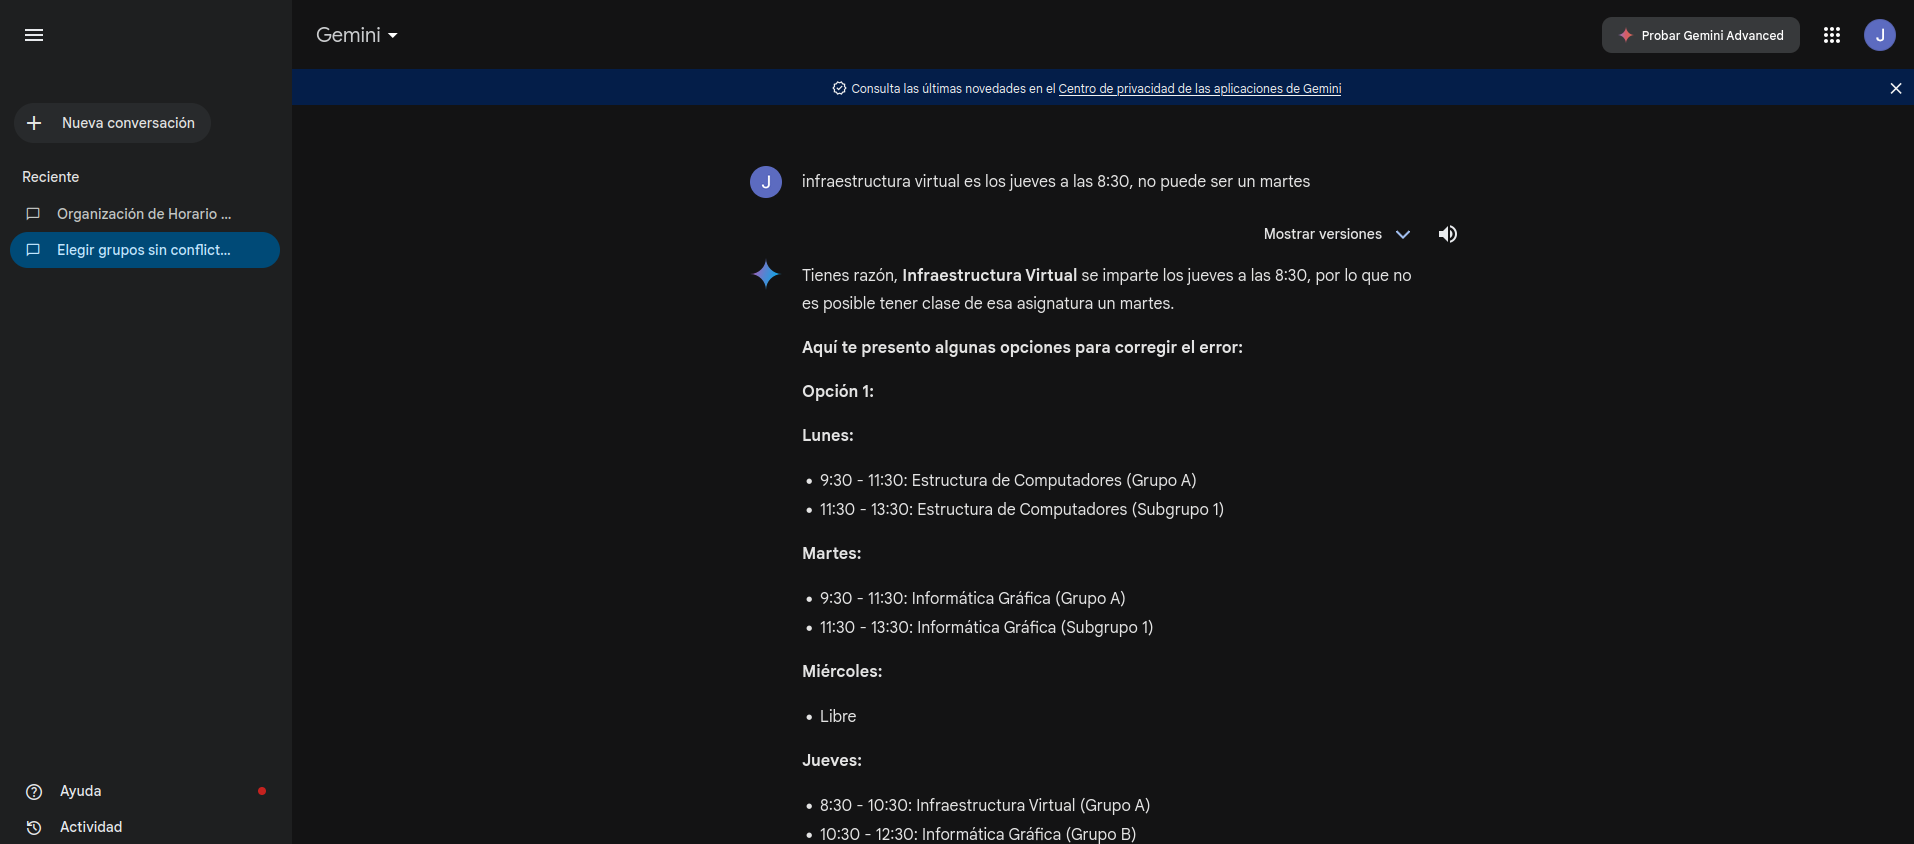
\includegraphics[width=1.5\textwidth, angle=0]{./imagenes/Gemini.png}
        \caption{Ejemplo con Gemini (Bard): omite asignaturas.}
    \end{figure}
\end{landscape}

\subsection{Proyectos académicos}

Además de las soluciones comerciales mencionadas, existen otros proyectos académicos que siguen el mismo enfoque:

\begin{enumerate}
    \item \textbf{Diego Barreiro Pérez}, \textit{Diseño e implementación de una aplicación web interactiva capaz de atender a preferencias y restricciones para la posterior generación automática de los horarios mediante heurísticas \cite{Barreiro}.}
\end{enumerate}

% A continuación se muestran imágenes de los asistentes mencionados:\newpage
% \begin{figure}[ht!]
%     \begin{minipage}{1\linewidth}
%         \centering
%         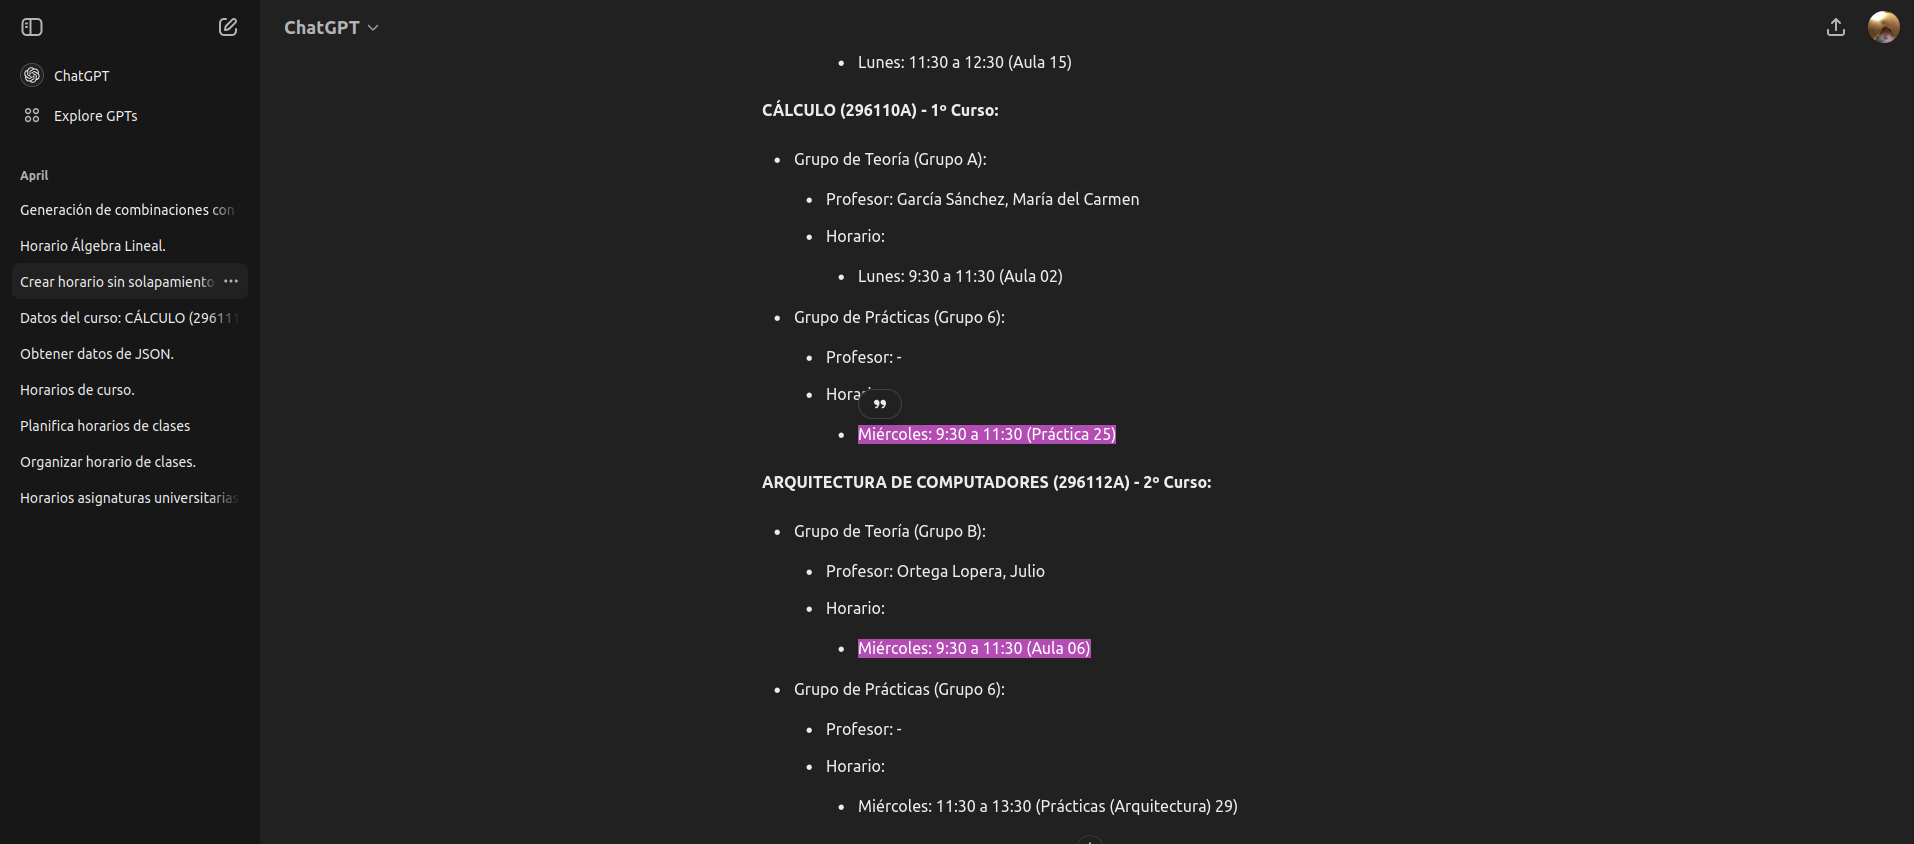
\includegraphics[width=\linewidth,height = 50mm]{./imagenes/ChatGPT.png}
%         \caption{Ejemplo con ChatGPT 3.5: solapa las clases.}
%         \vspace{0.5cm}
%     \end{minipage}
%     \begin{minipage}{1\linewidth}
%         \centering
%         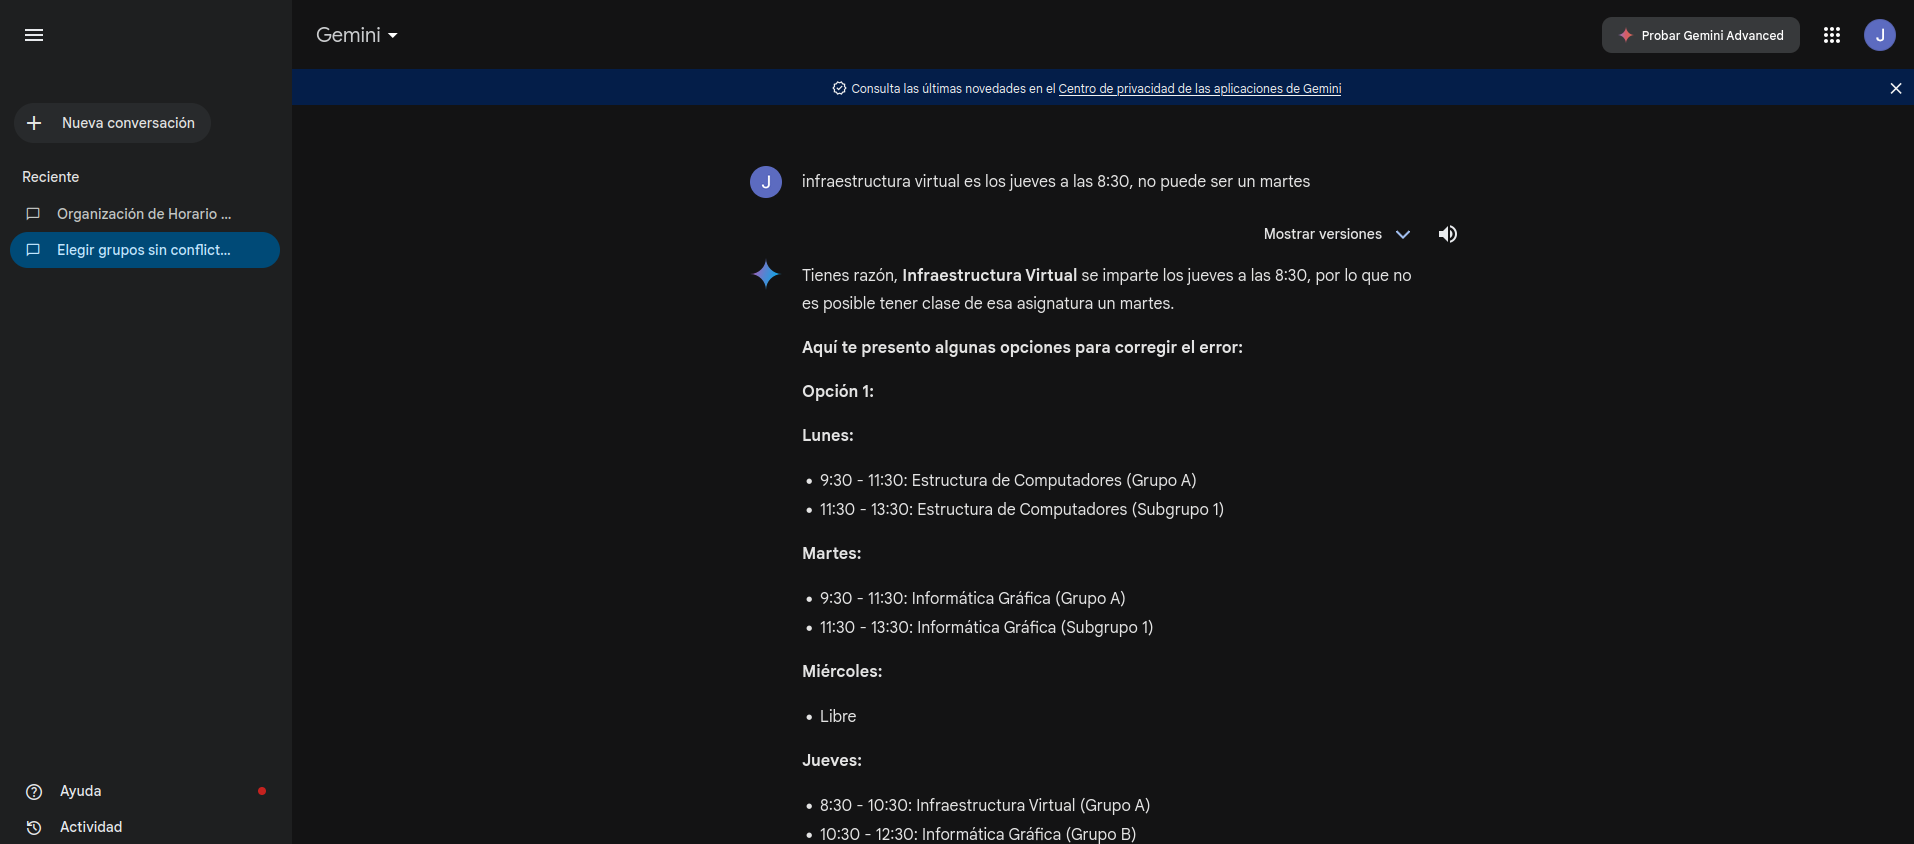
\includegraphics[width=\linewidth,height = 50mm]{./imagenes/Gemini.png}
%         \caption{Ejemplo con Gemini (Bard): omite asignaturas.}
%     \end{minipage}
% \end{figure}



% Existen múltiples estudios sobre algoritmos de timetabling para clases y exámenes universitarios:\\

Las aplicaciones discutidas anteriormente, como Google Calendar y Microsoft Calendar, son aplicaciones de calendario que permiten a los usuarios programar eventos y recordatorios. Se caracterizan por ser de propósito general, fáciles de usar y accesibles en múltiples dispositivos. Cuentan además con la ventaja de poder ser compartidos con otros usuarios, lo que facilita la colaboración en la programación de eventos.\newline

Por otro lado, los chatbots como ChatGPT y Gemini son aplicaciones de inteligencia artificial que permiten a los usuarios interactuar con un sistema de diálogo. Estos son capaces de responder preguntas y realizar tareas específicas. Son útiles para la programación de eventos en un calendario, ya que permiten a los usuarios interactuar con el sistema de forma natural y conversacional.\newline

Sin embargo, todas estas soluciones tienen una serie de limitaciones que las inadecuadas para el problema propuesto. Entre ellas se incluyen:

\begin{enumerate}
    \item \textbf{Falta de automatización:} Los usuarios deben participar activamente en la organización de bloques para poder conformar el horario que se adecue a sus necesidades. Este proceso resulta ineficiente y tedioso.
    \item \textbf{Extracción de datos:} La información de los horarios de las asignaturas debe ser consultada e introducida manualmente por el usuario, lo que puede resultar en errores y omisiones.
\end{enumerate}